\documentclass[border=5pt]{standalone}
\usepackage[utf8]{inputenc}
\usepackage[T1]{fontenc}
\usepackage{tikz}
\usetikzlibrary{shapes.geometric,arrows.meta,positioning,calc}

\definecolor{eegcolor}{RGB}{66,133,244}
\definecolor{ragcolor}{RGB}{234,67,53}
\definecolor{fusioncolor}{RGB}{251,188,5}
\definecolor{llmcolor}{RGB}{52,168,83}

\begin{document}
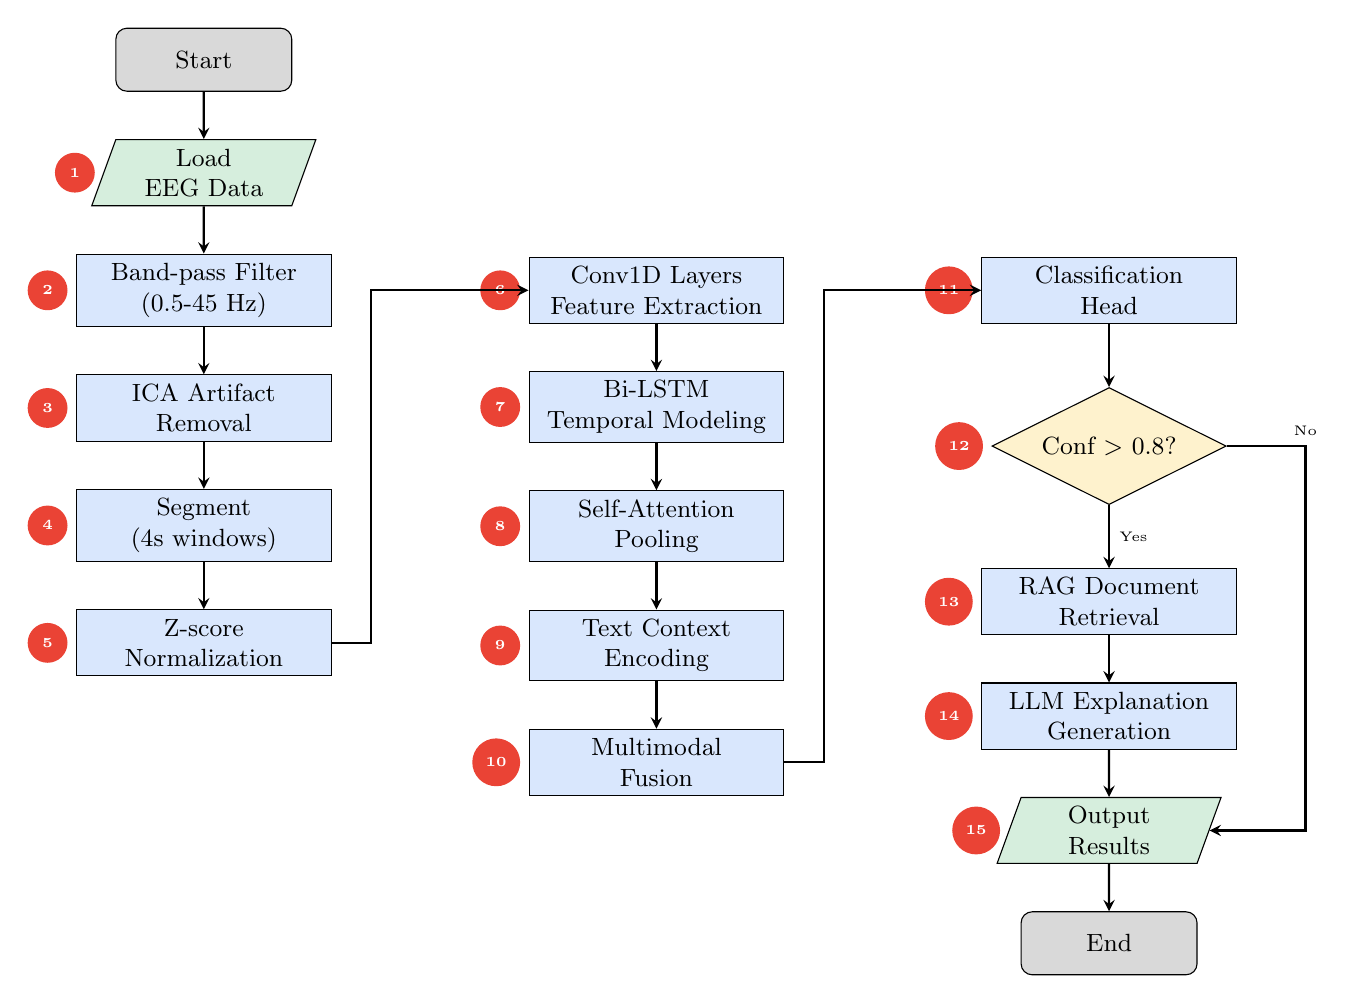
\begin{tikzpicture}[
    node distance=0.8cm,
    startstop/.style={rectangle, rounded corners, draw, fill=gray!30, text width=2cm, text centered, minimum height=0.8cm, font=\small},
    process/.style={rectangle, draw, fill=eegcolor!20, text width=3cm, text centered, minimum height=0.8cm, font=\small},
    decision/.style={diamond, draw, fill=fusioncolor!20, text width=1.8cm, text centered, minimum height=0.8cm, font=\small, aspect=2},
    io/.style={trapezium, trapezium left angle=70, trapezium right angle=110, draw, fill=llmcolor!20, text width=2cm, text centered, minimum height=0.6cm, font=\small},
    arrow/.style={->,>=stealth,thick},
    stepnum/.style={circle, fill=ragcolor, text=white, font=\tiny\bfseries, minimum size=0.5cm}
]

% Start
\node[startstop] (start) {Start};

% Step 1: Input
\node[io, below=0.6cm of start] (input) {Load EEG Data};
\node[stepnum, left=0.1cm of input] {1};

% Step 2: Preprocessing
\node[process, below=0.6cm of input] (preprocess) {Band-pass Filter\\(0.5-45 Hz)};
\node[stepnum, left=0.1cm of preprocess] {2};

% Step 3: Artifact Removal
\node[process, below=0.6cm of preprocess] (artifact) {ICA Artifact\\Removal};
\node[stepnum, left=0.1cm of artifact] {3};

% Step 4: Segmentation
\node[process, below=0.6cm of artifact] (segment) {Segment\\(4s windows)};
\node[stepnum, left=0.1cm of segment] {4};

% Step 5: Normalization
\node[process, below=0.6cm of segment] (normalize) {Z-score\\Normalization};
\node[stepnum, left=0.1cm of normalize] {5};

% Step 6: CNN Feature Extraction
\node[process, right=2.5cm of preprocess] (cnn) {Conv1D Layers\\Feature Extraction};
\node[stepnum, left=0.1cm of cnn] {6};

% Step 7: LSTM
\node[process, below=0.6cm of cnn] (lstm) {Bi-LSTM\\Temporal Modeling};
\node[stepnum, left=0.1cm of lstm] {7};

% Step 8: Attention
\node[process, below=0.6cm of lstm] (attention) {Self-Attention\\Pooling};
\node[stepnum, left=0.1cm of attention] {8};

% Step 9: Text Encoding
\node[process, below=0.6cm of attention] (textenc) {Text Context\\Encoding};
\node[stepnum, left=0.1cm of textenc] {9};

% Step 10: Fusion
\node[process, below=0.6cm of textenc] (fusion) {Multimodal\\Fusion};
\node[stepnum, left=0.1cm of fusion] {10};

% Step 11: Classification
\node[process, right=2.5cm of cnn] (classify) {Classification\\Head};
\node[stepnum, left=0.1cm of classify] {11};

% Step 12: Decision
\node[decision, below=0.8cm of classify] (decision) {Conf $>$ 0.8?};
\node[stepnum, left=0.1cm of decision] {12};

% Step 13: RAG Retrieval
\node[process, below=0.8cm of decision] (rag) {RAG Document\\Retrieval};
\node[stepnum, left=0.1cm of rag] {13};

% Step 14: LLM Generation
\node[process, below=0.6cm of rag] (llm) {LLM Explanation\\Generation};
\node[stepnum, left=0.1cm of llm] {14};

% Step 15: Output
\node[io, below=0.6cm of llm] (output) {Output Results};
\node[stepnum, left=0.1cm of output] {15};

% End
\node[startstop, below=0.6cm of output] (stop) {End};

% Arrows
\draw[arrow] (start) -- (input);
\draw[arrow] (input) -- (preprocess);
\draw[arrow] (preprocess) -- (artifact);
\draw[arrow] (artifact) -- (segment);
\draw[arrow] (segment) -- (normalize);
\draw[arrow] (normalize.east) -- ++(0.5,0) |- (cnn.west);
\draw[arrow] (cnn) -- (lstm);
\draw[arrow] (lstm) -- (attention);
\draw[arrow] (attention) -- (textenc);
\draw[arrow] (textenc) -- (fusion);
\draw[arrow] (fusion.east) -- ++(0.5,0) |- (classify.west);
\draw[arrow] (classify) -- (decision);
\draw[arrow] (decision) -- node[right, font=\tiny] {Yes} (rag);
\draw[arrow] (decision.east) -- ++(1,0) node[above, font=\tiny] {No} |- (output.east);
\draw[arrow] (rag) -- (llm);
\draw[arrow] (llm) -- (output);
\draw[arrow] (output) -- (stop);

\end{tikzpicture}
\end{document}
